\documentclass[leqno]{article}
% Shared QBT/Soln pack preamble for resources.danieljsmith.org.
\usepackage{graphicx}
\usepackage{dsfont}
\usepackage{mathtools}
\usepackage{amssymb}
\usepackage{amsmath}
\usepackage{mleftright}
\usepackage{amsthm}
\usepackage{float}
\usepackage{ragged2e}
\usepackage{tensor}
\usepackage{fancyhdr}
\usepackage{empheq}
\usepackage[most]{tcolorbox}
\usepackage{enumitem}
\usepackage{dirtytalk}
\usepackage{marginnote}
\usepackage{microtype}
\usepackage[
  a4paper,
  left=0.8in,
  right=1in,
  top=1in,
  bottom=0.5in,
  headheight=14pt,
  headsep=0.4in
]{geometry}
\setlength{\parindent}{0cm}

% TikZ / PGFPlots
\usepackage{pgfplots}
\pgfplotsset{compat=1.18}
\usepgfplotslibrary{fillbetween, polar}
\usetikzlibrary{calc, positioning}
\usetikzlibrary{angles, quotes}
\usetikzlibrary{arrows.meta}
\usetikzlibrary{decorations.pathreplacing, decorations.markings}
\usetikzlibrary{patterns}
\usetikzlibrary{intersections}

% Links and contents. The contents follow the TMUA papers: compact entries,
% no dot leaders, and each question's mark total in grey after its label.
\usepackage{tocloft}
\tocloftpagestyle{fancy}
\setlength{\cftbeforesubsecskip}{2pt}
\setlength{\cftsubsecindent}{1.5em}
\setlength{\cftsubsecnumwidth}{0pt}
\renewcommand{\cftsubsecfont}{\small\color{black}}
\renewcommand{\cftsubsecpagefont}{\small\color{black}}
\renewcommand{\cftsubsecleader}{\hfill}
\usepackage[colorlinks=true,linkcolor=black,citecolor=magenta,urlcolor=black]{hyperref}%
\urlstyle{same}

% Pack macros
% \marks also adds its value to the current question's total in the .aux
% file, so the contents show each total from the second pass. The write
% happens at shipout, so a box typeset more than once counts once. The
% pack's mark total for the contents-page title is summed the same way.
\makeatletter
\newcount\djs@totalmarks
\newcommand{\djsAddMarks}[2]{%
  \global\advance\djs@totalmarks#2\relax
  \@ifundefined{djs@marks@#1}%
    {\expandafter\xdef\csname djs@marks@#1\endcsname{#2}}%
    {\expandafter\xdef\csname djs@marks@#1\endcsname
      {\the\numexpr\csname djs@marks@#1\endcsname+#2\relax}}}
\RenewDocumentCommand{\marks}{o m}{%
  \protected@write\@auxout{}{\string\djsAddMarks{\number\value{enumi}}{#2}}%
  \IfValueTF{#1}%
    {\marginnote{\raggedright\textbf{[#2]}}[#1]}%
    {\marginnote{\raggedright\textbf{[#2]}}}%
}
\makeatother

\newcommand{\vspacerule}[2]{%
  \par\vspace*{#1}%
  \noindent\hrulefill\par
  \vspace*{#2}%
}

\definecolor{scarlet}{RGB}{205, 40, 75}
% Site colours for the contents-page title: the accent, the rule colour, a
% stronger rule colour for the path separator, and the muted text colour.
\definecolor{djsBurgundy}{RGB}{118, 59, 67}
\definecolor{djsHairline}{RGB}{216, 213, 205}
\definecolor{djsSlash}{RGB}{170, 166, 158}
\definecolor{djsMuted}{RGB}{96, 101, 106}

% Worked-solution box, adapted from the TMUA worked-solutions box. A white breakable box with a left scarlet rule and no surrounding
% frame or tint. A part that breaks fills the rest of its page, so the rule
% runs to the bottom margin; the unbroken or last part ends in a short
% horizontal foot rule so a solution visibly stops. Unlike the TMUA box there
% is no answer label. The box does not grow to the left, so the rule sits at
% the text edge; growing to the right keeps the usable line width close to the
% old tcolorbox Solution box.
% Spacing inside the box: paragraphs are 6pt apart, so source blank lines show
% (solutions put one after each display and none between a lead-in and its
% display). Every display gets 6pt above and 10pt below, whatever the length
% of its lead-in line; align rows are spread by an 8pt \jot; solution parts
% are 14pt apart and sub-parts 8pt; \left and \right space like ordinary
% brackets (mleftright); no single line is stranded at a page break; and
% neither the Solution label nor the line before a list ends a page. No
% skip can shrink, so full pages are not squeezed.
\newtcolorbox{djsSolution}{%
  enhanced, breakable, frame hidden, sharp corners, colback=white,
  height fixed for=first and middle, height fill,
  extras unbroken and last={natural height},
  borderline west={2.2pt}{0pt}{scarlet},
  left=11pt, right=0pt, top=5pt, bottom=13pt,
  before skip=13pt, after skip=4pt,
  grow to right by=10mm,
  overlay unbroken and last={%
    \fill[scarlet] (frame.south west)
      rectangle ([xshift=3.5cm, yshift=2.2pt]frame.south west);},
  before upper={{\color{scarlet}\bfseries Solution}\par\nobreak\vspace{4pt}%
    \setlength{\parskip}{6pt plus 2pt}%
    \setlength{\abovedisplayskip}{6pt plus 2pt}%
    \setlength{\abovedisplayshortskip}{6pt plus 2pt}%
    \setlength{\belowdisplayskip}{10pt plus 2pt}%
    \setlength{\belowdisplayshortskip}{10pt plus 2pt}%
    \setlength{\jot}{8pt}%
    \setlist{parsep=6pt plus 2pt, topsep=6pt plus 2pt, beginpenalty=10000}%
    \setlist[enumerate,1]{itemsep=14pt plus 2pt}%
    \setlist[enumerate,2]{itemsep=8pt plus 2pt}%
    \mleftright
    \clubpenalty=10000 \widowpenalty=10000 \displaywidowpenalty=10000\relax}}

% Optional smaller figure inside a solution box. \scalebox shrinks node text
% with the drawing. Not applied to existing figures.
\newcommand{\SolnFigureScale}{0.85}
\newsavebox{\djsSolnFigureBox}
\newenvironment{djsSolutionFigure}
  {\par\vspace{4pt}\begin{center}\begin{lrbox}{\djsSolnFigureBox}}
  {\end{lrbox}\scalebox{\SolnFigureScale}{\usebox{\djsSolnFigureBox}}%
   \end{center}\vspace{2pt}\par}

\newcommand{\cxl}[2]{%
  \tikz[baseline=(X.base)]{%
    \node[inner sep=0pt, outer sep=0pt, text=#1] (X) {$#2$};
    \draw[#1, line width=0.4pt] (X.south west)--(X.north east);
  }%
}

% Page-style hook run at the contents page and each question's opening page.
% A no-op for QBT packs; \djsSolnHeader points it at the fancy header.
\newcommand{\djsQuestionPageStyle}{}

% A contents entry: "Question N" in a box wide enough for two digits, so the
% mark totals line up, then the total in grey. Bookmarks keep "Question N".
\makeatletter
\newlength{\djsTocLabelWidth}
\newcommand{\djsTocMarks}[1]{%
  \@ifundefined{djs@marks@#1}{}{%
    {\footnotesize\itshape\color{black!45}%
     \csname djs@marks@#1\endcsname~mark%
     \ifnum\csname djs@marks@#1\endcsname=1 \else s\fi}}}
\newcommand{\djsTocEntry}[1]{%
  \texorpdfstring
    {\settowidth{\djsTocLabelWidth}{Question 00}%
     \makebox[\dimexpr\djsTocLabelWidth+0.9em\relax][l]{Question #1}%
     \djsTocMarks{#1}}%
    {Question #1}}
\makeatother

% The question count for the contents-page title is written to the .aux at
% the end of the document, so it also appears from the second pass.
\newcounter{djsQuestions}
\newcommand{\questionitem}{%
  \djsQuestionPageStyle
  \item\phantomsection
  \stepcounter{djsQuestions}%
  \addcontentsline{toc}{subsection}{\protect\djsTocEntry{\number\value{enumi}}}%
}
\makeatletter
\newcommand{\djsSetQuestionCount}[1]{\gdef\djs@questioncount{#1}}
\AtEndDocument{\immediate\write\@auxout
  {\string\djsSetQuestionCount{\number\value{djsQuestions}}}}
\makeatother

\renewcommand{\contentsname}{Questions}

% \djsPackHeader[<link content tag>]{<left header>}; the tag says which
% document a click on the header link came from.
\newcommand{\djsPackHeader}[2][questions]{%
  \pagestyle{fancy}%
  \fancyhead{}%
  \fancyfoot{}%
  \renewcommand{\headrulewidth}{0.9pt}%
  \lhead{#2}%
  \chead{}%
  \rhead{\href{https://danieljsmith.org/?utm_source=pdf&utm_campaign=further-maths&utm_content=#1}{danieljsmith.org}}%
}

% The header's topic is also the contents-page title, under which a label
% says which booklet this is.
\newcommand{\djsPackTitle}{}
\newcommand{\djsBookletLabel}{}
\newcommand{\djsQbtHeader}[1]{%
  \djsPackHeader{#1}%
  \renewcommand{\djsPackTitle}{#1}%
  \renewcommand{\djsBookletLabel}{Questions by topic}%
}

% The colophon at the foot of page one, independent of the page style: the
% contents-page title's hairline led by a short scarlet rule, then the date on
% the left and a link to the site on the right, all inside the bottom margin.
% Its sizes are fixed, so it matches the TMUA papers' colophon. The document
% supplies the date; recompiling never changes it.
\makeatletter
\newcommand{\djsLastUpdated}[1]{%
  \AtBeginDocument{\AddToHookNext{shipout/foreground}{\djs@colophon{#1}}}}
\newcommand{\djs@colophon}[1]{%
  \put(0.8in,-\dimexpr\paperheight-0.47in\relax){%
    \makebox[0pt][l]{\color{djsHairline}%
      \rule[0.9pt]{\dimexpr\paperwidth-1.8in\relax}{0.6pt}}%
    \makebox[0pt][l]{\color{scarlet}\rule{3.5cm}{2.2pt}}}%
  \put(0.8in,-\dimexpr\paperheight-0.32in\relax){\makebox[0pt][l]{%
    \fontsize{9}{11}\selectfont Last updated #1}}%
  \put(\dimexpr\paperwidth-1in\relax,-\dimexpr\paperheight-0.32in\relax){%
    \makebox[0pt][r]{\fontsize{7}{8.5}\selectfont\color{djsMuted}%
      Latest version at \href{https://resources.danieljsmith.org/}%
        {\color{black}resources.danieljsmith.org}}}}
\makeatother

% Solutions packs show the header only on the contents page and each
% question's opening page, so it never appears part-way through a solution.
% \thispagestyle marks the next page shipped out, which is the question's
% page because every solution question starts after a \newpage.
\newcommand{\djsSolnHeader}[1]{%
  \djsPackHeader[solutions]{\textit{Solutions} - #1}%
  \pagestyle{empty}%
  \renewcommand{\djsQuestionPageStyle}{\thispagestyle{fancy}}%
  \renewcommand{\djsPackTitle}{#1}%
  \renewcommand{\djsBookletLabel}{Worked solutions}%
}

% \djsSitePath{<strand>}{<topic>}, called once after the header, names where
% the pack sits on the site; the contents-page title prints it above the pack
% title, e.g. CORE PURE / FURTHER CALCULUS. Without it the line is left out.
\makeatletter
\newif\ifdjs@sitepath
\newcommand{\djs@strand}{}
\newcommand{\djs@section}{}
\newcommand{\djsSitePath}[2]{%
  \djs@sitepathtrue
  \renewcommand{\djs@strand}{#1}%
  \renewcommand{\djs@section}{#2}%
}
\makeatother

% Further Mechanics packs call \djsMechanicsPack in their preamble, so that
% \djsFrontMatter prints the default value of g above the contents. The box
% keeps its own space above it (before skip is the whole gap below the title,
% not an addition to it). Without the box, \djsGravityNote is just extra space
% before the contents heading, bringing the gap above it close to the gap
% between the box and the heading on Further Mechanics pages.
\newcommand{\djsGravityNote}{\vspace{14pt}}
\newcommand{\djsMechanicsPack}{%
  \renewcommand{\djsGravityNote}{%
    \begin{tcolorbox}[sharp corners, colback=white, colframe=black,
      boxrule=1pt, left=8pt, right=8pt, top=6pt, bottom=6pt,
      before skip=20pt]
    {\bfseries Instructions}\par\vspace{4pt}
    Unless a question states otherwise, take $g = 9.8\,\mathrm{m\,s^{-2}}$
    wherever a numerical value of $g$ is required. Solutions also give final
    answers for $g = 10\,\mathrm{m\,s^{-2}}$ where these differ.
    \end{tcolorbox}%
    \vspace{16pt}}%
}

% Contents-page title: the site path in spaced burgundy capitals, the pack
% title, a hairline led by a short scarlet rule (the solution box's foot rule),
% then the booklet label with the question and mark counts. The counts come
% from the .aux, so they appear from the second pass.
\makeatletter
\newsavebox{\djs@eyebrowbox}
\newcommand{\djs@caps}[1]{\textls[180]{\MakeUppercase{#1}}}
\newcommand{\djs@eyebrow}{%
  \color{djsBurgundy}\footnotesize\bfseries
  \djs@caps{\djs@strand}%
  {\color{djsSlash}\hspace{0.55em}/\hspace{0.55em}}%
  \djs@caps{\djs@section}}
\newcommand{\djs@dot}{\hspace{0.45em}\textperiodcentered\hspace{0.45em}}
\newcommand{\djs@counts}{%
  \@ifundefined{djs@questioncount}{}{%
    \djs@questioncount~question\ifnum\djs@questioncount=1 \else s\fi
    \ifnum\djs@totalmarks>0
      \djs@dot\the\djs@totalmarks~mark\ifnum\djs@totalmarks=1 \else s\fi
    \fi}}
\newcommand{\djsContentsTitle}{%
  \ifdjs@sitepath
    \sbox\djs@eyebrowbox{\djs@eyebrow}%
    \ifdim\wd\djs@eyebrowbox>\linewidth
      \@latex@warning@no@line{The \string\djsSitePath\space line is wider
        than the text, so it wraps. Shorten its topic}%
    \fi
    {\raggedright\djs@eyebrow\par}%
    \vspace{7pt}%
  \fi
  {\raggedright\fontsize{24.88}{28}\selectfont\djsPackTitle\par}%
  \vspace{9pt}%
  \noindent\makebox[0pt][l]{\color{djsHairline}\rule[0.9pt]{\linewidth}{0.6pt}}%
  {\color{scarlet}\rule{3.5cm}{2.2pt}}\par
  \vspace{5pt}%
  {\small\color{djsMuted}\djsBookletLabel\hfill\djs@counts\par}%
  \vspace{8pt}%
}
\makeatother

\newcommand{\djsFrontMatter}{%
  \djsQuestionPageStyle
  \vspace*{6pt}%
  \djsContentsTitle
  \djsGravityNote
  \tableofcontents
  \newpage
}


\djsSolnHeader{Polar Coordinates Basics}
\djsSitePath{Core Pure}{Polar Coordinates}
\djsLastUpdated{25 October 2026}

\begin{document}
\djsFrontMatter
\begin{enumerate}[
  label=\textbf{\arabic*.},
  leftmargin=*,
  topsep=0pt,
  partopsep=0pt,
  parsep=0pt
]

% ---- Question 1 ----
\questionitem
% [Source: _QBT___Solns__Polar_Coordinates_Basics, Q1]

\begin{figure}[H]
    \centering
\begin{tikzpicture}[scale=1.5]
\def\displayunit{0.35}
\def\rstart{1}
\def\growth{2}
\def\outerradius{8}
\pgfmathsetmacro{\tmax}{pi}
\pgfmathsetmacro{\endpoint}{\displayunit*(\rstart+\growth*\tmax)}
\pgfmathsetmacro{\axisend}{1.2*\displayunit*\outerradius}
\pgfmathsetmacro{\workspace}{1.15*\displayunit*\outerradius}
\coordinate (O) at (0,0);
\coordinate (A) at (180:\endpoint);
\coordinate (L) at (\axisend,0);
\path[use as bounding box] (-\workspace,-\workspace) rectangle (\axisend,\workspace);
\draw[thick, black, samples=200, domain=0:\tmax, variable=\t]
  plot ({\displayunit*(\rstart+\growth*\t)*cos(deg(\t))},{\displayunit*(\rstart+\growth*\t)*sin(deg(\t))});
\draw[-{Stealth[length=3mm]}, thick, black] (O) -- (L);
\fill[black] (O) circle (1.5pt);
\node[below left=2pt] at (O) {$O$};
\node[left=2pt] at (A) {$A$};
\node[below] at (L) {Initial line};
\end{tikzpicture}
\end{figure}


The polar curves $C_1$ and $C_2$ are defined by
\[
C_1: r=1+2\theta,\qquad 0\leqslant\theta\leqslant\pi
\] \\
and
\[
C_2: r=8-\theta,\qquad 0\leqslant\theta\leqslant2\pi
\] \\
The diagram above shows $C_1$. Its endpoint $A$ lies on the ray opposite the initial line. \\
\begin{enumerate}[label=\textbf{(\alph*)}]
\item State the polar coordinates of $A$ and find its Cartesian coordinates, taking the pole as the origin and the initial line as the positive $x$-axis. \marks{3} \\
\item Find the polar coordinates of the point where $C_1$ and $C_2$ intersect. \marks{2} \\
\item On a copy of the diagram above, sketch $C_2$, indicating the radii of its two endpoints. \marks{3} \\
\end{enumerate}

\vspace*{10pt}

\begin{djsSolution}
\begin{enumerate}[label=\textbf{(\alph*)}, start=1]
\item
The ray opposite the initial line has \(\theta=\pi\), giving \(r=1+2\pi\). Hence the polar coordinates of \(A\) are
\[
(1+2\pi,\pi)
\]

Using \(x=r\cos\theta\) and \(y=r\sin\theta\):
\begin{align*}
x&=(1+2\pi)\cos\pi=-1-2\pi\\
y&=(1+2\pi)\sin\pi=0
\end{align*}

Thus the Cartesian coordinates of \(A\) are
\[
(-1-2\pi,0)
\]

\item At the intersection, the two radii are equal:
\begin{align*}
1+2\theta&=8-\theta\\
3\theta&=7\quad\Longrightarrow\quad\theta=\dfrac73\\
r&=1+2\left(\dfrac73\right)=\dfrac{17}{3}
\end{align*}

The polar coordinates of the intersection are
\[
\left(\dfrac{17}{3},\dfrac73\right)
\]

\item The sketch should look like:\par\nopagebreak

\begin{tikzpicture}[scale=0.75]
\def\rOuter{8}
\def\rStart{1}
\def\growth{2}
\pgfmathsetmacro{\thOne}{pi}
\pgfmathsetmacro{\thTwo}{2*pi}
\pgfmathsetmacro{\rInner}{\rOuter-\thTwo}
\pgfmathsetmacro{\rA}{\rStart+\growth*\thOne}
\pgfmathsetmacro{\axisEnd}{1.15*\rOuter}
\pgfmathsetmacro{\labelOne}{\rStart+\growth*pi/2}
\pgfmathsetmacro{\labelTwo}{\rOuter-pi/2}
\coordinate (O) at (0,0);
\coordinate (A) at (180:\rA);
\coordinate (S) at (0:\rOuter);
\coordinate (T) at (0:\rInner);
\coordinate (L) at (\axisEnd,0);
\coordinate (LabelOne) at (90:\labelOne);
\coordinate (LabelTwo) at (90:\labelTwo);
\draw[thick, black, samples=150, domain=0:\thOne, variable=\t]
  plot ({(\rStart+\growth*\t)*cos(deg(\t))},{(\rStart+\growth*\t)*sin(deg(\t))});
\draw[thick, black, samples=200, domain=0:\thTwo, variable=\t]
  plot ({(\rOuter-\t)*cos(deg(\t))},{(\rOuter-\t)*sin(deg(\t))});
\draw[-{Stealth[length=3mm]}, thick, black] (O) -- (L);
\node[below left=2pt] at (O) {$O$};
\node[left=2pt] at (A) {$A$};
\node[below right] at (L) {Initial line};
\node[below left] at (LabelOne) {$C_1$};
\node[above right] at (LabelTwo) {$C_2$};
\foreach \P in {S,T} {\fill[black] (\P) circle (1.5pt);}
\node[above right=2pt] at (S) {$(8,0)$};
\node[below right=2pt] at (T) {$(8-2\pi,2\pi)$};
\end{tikzpicture}

As \(\theta\) increases, \(C_2\) makes one anticlockwise turn inwards, with endpoint radii \(8\) and \(8-2\pi\).
\end{enumerate}
\end{djsSolution}

\newpage

% ---- Question 2 ----
\questionitem
% [Source: _QBT___Solns__Polar_Coordinates_Basics, Q2]

The curve $C$ has the polar equation
\[
r=\frac{6}{2-\sin\theta},\qquad -\pi<\theta\leq\pi
\] \\
\begin{enumerate}[label=\textbf{(\alph*)}]
\item Verify that the point with polar coordinates $\left(4,\frac{\pi}{6}\right)$ lies on $C$. \marks{1} \\
\item Find the exact polar coordinates of the point on $C$ which is furthest from the pole, $O$. \marks{3} \\
\item The Cartesian line $y=x$ intersects $C$ at two points. Find the exact Cartesian coordinates of both points. \marks{4} \\
\end{enumerate}

\vspace*{10pt}

\begin{djsSolution}
\begin{enumerate}[label=\textbf{(\alph*)}, start=1]
\item Substituting \(\theta=\frac{\pi}{6}\) into the polar equation gives
\[
r=\dfrac{6}{2-\sin\frac{\pi}{6}}=\dfrac{6}{2-\frac12}=4
\]

Thus \(\left(4,\frac{\pi}{6}\right)\) lies on \(C\).

\item Since \(-1\leq\sin\theta\leq1\), it follows that
\[
1\leq 2-\sin\theta\leq3
\quad\Longrightarrow\quad
2\leq r\leq6
\]

As \(r>0\), the distance from the pole is \(r\). The greatest distance is therefore \(6\), attained when \(\sin\theta=1\), so \(\theta=\frac{\pi}{2}\) in the given interval. The required polar coordinates are
\[
\left(6,\dfrac{\pi}{2}\right)
\]

\item Using \(x=r\cos\theta\) and \(y=r\sin\theta\), the line \(y=x\) gives
\begin{align*}
r\sin\theta&=r\cos\theta\\
\sin\theta&=\cos\theta \qquad (r>0)\\
\tan\theta&=1\\
\theta&=\dfrac{\pi}{4}\quad\text{or}\quad-\dfrac{3\pi}{4}
\end{align*}

At \(\theta=\frac{\pi}{4}\):
\begin{align*}
r&=\dfrac{6}{2-\frac{\sqrt2}{2}}=\dfrac{12}{4-\sqrt2}\\
x=y&=\dfrac{12}{4-\sqrt2}\times\dfrac{\sqrt2}{2}
=\dfrac{6\sqrt2(4+\sqrt2)}{16-2}
=\dfrac{6+12\sqrt2}{7}
\end{align*}

At \(\theta=-\frac{3\pi}{4}\):
\begin{align*}
r&=\dfrac{6}{2+\frac{\sqrt2}{2}}=\dfrac{12}{4+\sqrt2}\\
x=y&=\dfrac{12}{4+\sqrt2}\times\left(-\dfrac{\sqrt2}{2}\right)
=-\dfrac{6\sqrt2(4-\sqrt2)}{16-2}
=\dfrac{6-12\sqrt2}{7}
\end{align*}

The Cartesian coordinates of the two points are
\[
\left(\dfrac{6+12\sqrt2}{7},\dfrac{6+12\sqrt2}{7}\right)
\quad\text{and}\quad
\left(\dfrac{6-12\sqrt2}{7},\dfrac{6-12\sqrt2}{7}\right)
\]

\end{enumerate}
\end{djsSolution}

\newpage

% ---- Question 3 ----
\questionitem
% [Source: _QBT___Solns__Polar_Coordinates_Basics, Q3]

\begin{figure}[H]
    \centering
\begin{tikzpicture}[scale=1.5, x=0.65cm, y=0.65cm]
\def\base{4}
\def\amp{3}
\def\axislen{2.5}
\def\leftspace{7.5}
\def\rightspace{3.5}
\def\verticalspace{5.3}
\coordinate (O) at (0,0);
\coordinate (InitialEnd) at (\axislen,0);
\path[use as bounding box] (-\leftspace,-\verticalspace) rectangle (\rightspace,\verticalspace);
\draw[thick, black, domain=0:180, samples=200, variable=\t]
  plot ({(\base-\amp*cos(\t))*cos(\t)},{(\base-\amp*cos(\t))*sin(\t)});
\draw[-{Stealth[length=3mm]}, thick, black] (O) -- (InitialEnd)
  node[right] {Initial line};
\node[left] at (O) {$O$};
\end{tikzpicture}
\end{figure}


The curve $C$ has polar equation
\[
r=4-3\cos\theta,\qquad -\pi<\theta\leq\pi
\] \\
\begin{enumerate}[label=\textbf{(\alph*)}]
\item The diagram above shows the portion of $C$ for which $0\leq\theta\leq\pi$. Complete the sketch of $C$. \marks{1} \\
\end{enumerate}
The straight line $\ell$ has polar equation
\[
r\cos\theta=1
\] \\
\begin{enumerate}[label=\textbf{(\alph*)}, resume]
\item Add $\ell$ to your completed sketch and find all the points of intersection of $C$ and $\ell$. Give their polar coordinates, with radii exact and any non-zero angles in radians to $3$ significant figures. \marks{6} \\
\end{enumerate}

\vspace*{10pt}

\begin{djsSolution}
\begin{enumerate}[label=\textbf{(\alph*)}, start=1]
\item
The completed sketch should look like:\par\nopagebreak

\begin{tikzpicture}[scale=0.85]
\def\base{4}
\def\amp{3}
\def\axislen{2.5}
\def\leftspace{7.5}
\def\rightspace{3.5}
\def\verticalspace{5.3}
\coordinate (O) at (0,0);
\coordinate (InitialEnd) at (\axislen,0);
\path[use as bounding box] (-\leftspace,-\verticalspace) rectangle (\rightspace,\verticalspace);
\draw[thick, black, domain=-180:180, samples=300, variable=\t]
  plot ({(\base-\amp*cos(\t))*cos(\t)},{(\base-\amp*cos(\t))*sin(\t)});
\draw[-{Stealth[length=3mm]}, thick, black] (O) -- (InitialEnd)
  node[right] {Initial line};
\node[below left=2pt] at (O) {$O$};
\end{tikzpicture}

Since \(\cos(-\theta)=\cos\theta\), the curve is symmetric about the initial line. Reflect the given portion in the initial line to complete \(C\).

\item The sketch with \(\ell\) added should look like:\par\nopagebreak

\begin{tikzpicture}[scale=0.85]
\def\base{4}
\def\amp{3}
\def\axislen{2.5}
\def\leftspace{7.5}
\def\rightspace{3.5}
\def\verticalspace{5.3}
\def\lineX{1}
\pgfmathsetmacro{\interR}{\base-\amp/3}
\pgfmathsetmacro{\interAng}{acos(1/3)}
\coordinate (O) at (0,0);
\coordinate (InitialEnd) at (\axislen,0);
\coordinate (LineBottom) at (\lineX,-\verticalspace);
\coordinate (LineTop) at (\lineX,\verticalspace);
\coordinate (IntersectionZero) at (\lineX,0);
\coordinate (IntersectionUpper) at (\interAng:\interR);
\coordinate (IntersectionLower) at (-\interAng:\interR);
\path[use as bounding box] (-\leftspace,-\verticalspace) rectangle (\rightspace,\verticalspace);
\draw[thick, black, domain=-180:180, samples=300, variable=\t]
  plot ({(\base-\amp*cos(\t))*cos(\t)},{(\base-\amp*cos(\t))*sin(\t)});
\draw[thick, black] (LineBottom) -- (LineTop) node[above right] {$\ell$};
\draw[-{Stealth[length=3mm]}, thick, black] (O) -- (InitialEnd)
  node[right] {Initial line};
\node[below left=2pt] at (O) {$O$};
\foreach \P in {IntersectionZero,IntersectionUpper,IntersectionLower}
  {\fill[black] (\P) circle (1.5pt);}
\node[above right=3pt] at (IntersectionZero) {$(1,0)$};
\node[above right=3pt] at (IntersectionUpper) {$(3,1.23)$};
\node[below right=3pt] at (IntersectionLower) {$(3,-1.23)$};
\end{tikzpicture}

Since \(x=r\cos\theta\), the equation of \(\ell\) is \(x=1\), so it is a vertical line through \((1,0)\).

At an intersection, substitute \(r=4-3\cos\theta\) into the equation of \(\ell\):
\begin{align*}
(4-3\cos\theta)\cos\theta&=1\\
3\cos^2\theta-4\cos\theta+1&=0\\
(3\cos\theta-1)(\cos\theta-1)&=0
\end{align*}

Thus \(\cos\theta=1\) or \(\cos\theta=\frac13\). In the given range \(-\pi<\theta\leq\pi\), these give
\begin{align*}
\cos\theta=1&\quad\Longrightarrow\quad \theta=0,\qquad r=4-3=1\\
\cos\theta=\dfrac13&\quad\Longrightarrow\quad
\theta=\pm\arccos\left(\dfrac13\right),\qquad
r=4-3\left(\dfrac13\right)=3
\end{align*}

The polar coordinates are
\[
(1,0),\qquad (3,1.23),\qquad (3,-1.23)\qquad\text{(3 s.f.)}
\]

\end{enumerate}
\end{djsSolution}

\newpage

% ---- Question 4 ----
\questionitem
% [Source: _QBT___Solns__Polar_Coordinates_Basics, Q4]

The curve $C_1$ has polar equation
\[
r^2+4r\cos\theta-6r\sin\theta=12
\] \\
where $r>0$ and $-\pi<\theta\leq\pi$. \\
\begin{enumerate}[label=\textbf{(\alph*)}]
\item Find a Cartesian equation for $C_1$ and show that it represents a circle. State its radius and the Cartesian coordinates of its centre. \marks{4} \\
\item Sketch $C_1$, marking its centre and the pole. Find the exact greatest and least distances of a point on $C_1$ from the pole. \marks{4} \\
\end{enumerate}

\vspace*{10pt}

\begin{djsSolution}
\begin{enumerate}[label=\textbf{(\alph*)}, start=1]
\item Using \(x=r\cos\theta\), \(y=r\sin\theta\) and \(r^2=x^2+y^2\), the polar equation becomes
\begin{align*}
x^2+y^2+4x-6y&=12\\
(x^2+4x+4)+(y^2-6y+9)&=12+4+9\\
(x+2)^2+(y-3)^2&=25
\end{align*}

This has the standard circle form \((x-a)^2+(y-b)^2=R^2\), so
\[
\text{Centre }(-2,3),\qquad \text{radius }5
\]

\item The sketch should look like:\par\nopagebreak

\begin{tikzpicture}
\begin{axis}[
width=0.8\linewidth,
height=8cm,
axis lines=middle,
axis equal image,
xmin=-8, xmax=4,
ymin=-3, ymax=9,
xtick=\empty,
ytick=\empty,
xlabel={$x$},
ylabel={$y$},
clip=false
]
\addplot[domain=0:360,samples=181,smooth] ({-2+5*cos(x)},{3+5*sin(x)});
\fill (axis cs:-2,3) circle (2pt);
\node[anchor=east] at (axis cs:-2.2,3) {\((-2,3)\)};
\fill (axis cs:0,0) circle (2pt);
\node[anchor=north east] at (axis cs:-0.15,-0.15) {\(O(0,0)\)};
\node at (axis cs:2.4,6.6) {\(C_1\)};
\end{axis}
\end{tikzpicture}

The distance of a point on \(C_1\) from the pole is \(r\), since \(r>0\). The centre \(A\) has Cartesian coordinates \((-2,3)\), so its distance from the pole is
\[
OA=\sqrt{(-2)^2+3^2}=\sqrt{13}
\]

Since \(\sqrt{13}<5\), the pole lies inside the circle. The line through \(A\) and \(O\) meets \(C_1\) at the furthest point \(F\), beyond \(A\), and at the nearest point \(N\), beyond \(O\):\par\nopagebreak

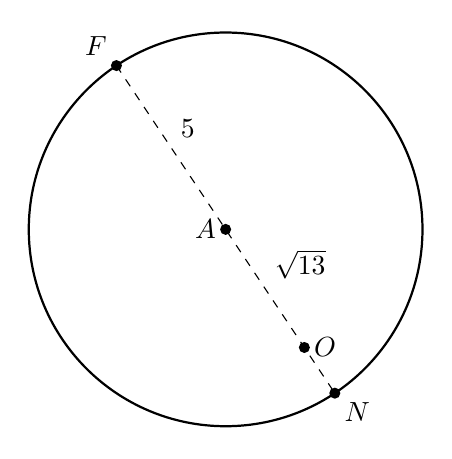
\begin{tikzpicture}[x=0.5cm,y=0.5cm]
\coordinate (O) at (0,0);
\coordinate (A) at (-2,3);
\coordinate (F) at ({-2-10/sqrt(13)},{3+15/sqrt(13)});
\coordinate (N) at ({-2+10/sqrt(13)},{3-15/sqrt(13)});
\draw[thick] (A) circle (5);
\draw[dashed] (F) -- (N);
\foreach \p in {O,A,F,N} \fill (\p) circle (2pt);
\node[left] at (A) {\(A\)};
\node[right] at (O) {\(O\)};
\node[above left] at (F) {\(F\)};
\node[below right] at (N) {\(N\)};
\node[above right] at ($(A)!0.5!(F)$) {\(5\)};
\node[above right] at ($(O)!0.5!(A)$) {\(\sqrt{13}\)};
\end{tikzpicture}

From the diagram, the extremes are at \(F\) and \(N\):
\begin{align*}
\text{Greatest distance}=OF&=OA+AF=5+\sqrt{13}\\
\text{Least distance}=ON&=AN-OA=5-\sqrt{13}
\end{align*}

\end{enumerate}
\end{djsSolution}

\newpage

% ---- Question 5 ----
\questionitem
% [Source: _QBT___Solns__Polar_Coordinates_Basics, Q5]

\begin{enumerate}[label=\textbf{(\alph*)}]
\item The curve $C_1$ has Cartesian equation
\[
x^2+y^2=\sqrt{3}\,y
\] \\
Find the centre and radius of $C_1$, and show that its non-pole points have polar equation $r=\sqrt{3}\sin\theta$. \marks{4} \\
\end{enumerate}
The curve $C_2$ has polar equation
\[
r=1+\cos\theta
\] \\
Consider both curves for $0<\theta<\pi$, together with their limiting endpoints. \\
In this interval, $r>0$ for both curves. The pole is a limiting endpoint of each curve. \\
\begin{enumerate}[label=\textbf{(\alph*)}, resume]
\item Show that $C_1$ and $C_2$ have exactly one intersection other than the pole, and find the exact polar coordinates of this intersection, $P$. \marks{4} \\
\item Sketch both curves on a single diagram, clearly labelling each curve. Mark $P$ and indicate the Cartesian coordinates of every point where either curve meets the initial line. \marks{3} \\
\end{enumerate}

\vspace*{10pt}

\begin{djsSolution}
\begin{enumerate}[label=\textbf{(\alph*)}, start=1]
\item Completing the square:
\begin{align*}
x^2+y^2-\sqrt{3}\,y&=0\\
x^2+\left(y-\dfrac{\sqrt{3}}{2}\right)^2&=\dfrac{3}{4}
\end{align*}

Hence the centre and radius are
\[
\text{Centre }\left(0,\dfrac{\sqrt{3}}{2}\right),\qquad
\text{radius }\dfrac{\sqrt{3}}{2}
\]

Substituting \(x=r\cos\theta\) and \(y=r\sin\theta\) into the original equation:
\begin{align*}
r^2\cos^2\theta+r^2\sin^2\theta&=\sqrt{3}\,r\sin\theta\\
r^2&=\sqrt{3}\,r\sin\theta
\end{align*}

At a non-pole point, \(r\ne0\), so division by \(r\) gives
\[
r=\sqrt{3}\sin\theta
\]

\item Since both radii are positive for \(0<\theta<\pi\), a non-pole intersection must have equal radii at the same angle:
\begin{align*}
\sqrt{3}\sin\theta&=1+\cos\theta\\
\sqrt{3}\sin\theta-\cos\theta&=1
\end{align*}

Write \(\sqrt{3}\sin\theta-\cos\theta\) in the form \(R\sin(\theta-\alpha)\), where \(R>0\) and \(0<\alpha<\frac{\pi}{2}\). Expanding:
\[
R\sin(\theta-\alpha)=R\sin\theta\cos\alpha-R\cos\theta\sin\alpha
\]

Comparing the coefficients of \(\sin\theta\) and \(\cos\theta\):
\[
R\cos\alpha=\sqrt{3},\qquad R\sin\alpha=1
\]

so
\[
R=\sqrt{\left(\sqrt{3}\right)^2+1^2}=2,\qquad
\tan\alpha=\dfrac{1}{\sqrt{3}}
\quad\Longrightarrow\quad
\alpha=\dfrac{\pi}{6}
\]

Hence the equation becomes
\begin{align*}
2\sin\left(\theta-\dfrac{\pi}{6}\right)&=1\\
\sin\left(\theta-\dfrac{\pi}{6}\right)&=\dfrac12
\end{align*}

For \(0\leq\theta\leq\pi\), this gives
\[
\theta-\dfrac{\pi}{6}=\dfrac{\pi}{6}\quad\text{or}\quad\dfrac{5\pi}{6},
\qquad\text{so}\qquad
\theta=\dfrac{\pi}{3}\quad\text{or}\quad\pi
\]

The value \(\theta=\pi\) is the pole endpoint and is excluded from the interval. Therefore there is exactly one non-pole intersection. Its radius is
\[
r=1+\cos\dfrac{\pi}{3}=\dfrac32
\]

so \(P\) has polar coordinates
\[
\left(\dfrac32,\dfrac{\pi}{3}\right)
\]

\item The sketch should look like:\par\nopagebreak

\begin{tikzpicture}[x=3.2cm,y=3.2cm]
\draw[->] (-1.2,0) -- (2.5,0) node[right] {\(x\)};
\draw[->] (0,-0.3) -- (0,2.1) node[above] {\(y\)};
\draw[domain=0:180,samples=181,smooth,variable=\t]
  plot ({sqrt(3)*sin(\t)*cos(\t)},{sqrt(3)*sin(\t)*sin(\t)});
\draw[domain=0:180,samples=181,smooth,variable=\t]
  plot ({(1+cos(\t))*cos(\t)},{(1+cos(\t))*sin(\t)});
\node at (-0.85,1.55) {\(C_1\)};
\node at (1.95,0.8) {\(C_2\)};
\fill (0,0) circle (1.5pt);
\node[below left] at (0,0) {\((0,0)\)};
\fill (2,0) circle (1.5pt);
\node[below] at (2,0) {\((2,0)\)};
\fill (0.75,{3*sqrt(3)/4}) circle (1.5pt);
\node[above right] at (0.75,{3*sqrt(3)/4}) {\(P\left(\frac32,\frac{\pi}{3}\right)\)};
\end{tikzpicture}

\(C_1\) is the full circle from part (a), lying above the initial line and touching it at the pole. At both limiting endpoints, \(r=\sqrt{3}\sin\theta=0\), so its only point on the initial line has Cartesian coordinates \((0,0)\).

\(C_2\) is the upper half of the cardioid, extending slightly into \(x<0\) before reaching the pole. Since \(r(0)=2\) and \(r(\pi)=0\), its points on the initial line have Cartesian coordinates \((2,0)\) and \((0,0)\).
\end{enumerate}
\end{djsSolution}

\newpage

% ---- Question 6 ----
\questionitem
% [Source: _QBT___Solns__Polar_Coordinates_Basics, Q6]

A curve has Cartesian equation
\[
(x^2+y^2)^2=5x^2+4xy+2y^2
\] \\
where $x$ and $y$ are not both zero. Use the convention $r>0$. \\
\begin{enumerate}[label=\textbf{(\roman*)}]
\item Show that the polar equation of the curve is
\[
r^2=\frac{7+3\cos 2\theta+4\sin 2\theta}{2}
\] \marks[-30pt]{4}
\item Hence find the least and greatest distances of points on the curve from the origin, giving your answers in exact form. \marks{3} \\
\end{enumerate}

\vspace*{10pt}

\begin{djsSolution}
\begin{enumerate}[label=\textbf{(\roman*)}, start=1]
\item Using \(x=r\cos\theta\), \(y=r\sin\theta\) and \(r^2=x^2+y^2\), the Cartesian equation becomes
\[
r^4=5r^2\cos^2\theta+4r^2\cos\theta\sin\theta+2r^2\sin^2\theta
\]

Since \(r>0\), we can divide by \(r^2\). Applying the double angle formulae gives
\begin{align*}
r^2&=5\cos^2\theta+4\cos\theta\sin\theta+2\sin^2\theta\\
&=\dfrac{5}{2}(1+\cos2\theta)+2\sin2\theta+(1-\cos2\theta)\\
&=\dfrac{7}{2}+\dfrac{3}{2}\cos2\theta+2\sin2\theta\\
&=\dfrac{7+3\cos2\theta+4\sin2\theta}{2}
\end{align*}

\item Write \(3\cos2\theta+4\sin2\theta\) in the form \(R\cos(2\theta-\alpha)\), where \(R>0\) and \(0<\alpha<\frac{\pi}{2}\). Expanding:
\[
R\cos(2\theta-\alpha)=R\cos2\theta\cos\alpha+R\sin2\theta\sin\alpha
\]

Comparing the coefficients of \(\cos2\theta\) and \(\sin2\theta\):
\[
R\cos\alpha=3,\qquad R\sin\alpha=4
\]

so
\[
R=\sqrt{3^2+4^2}=5,\qquad \tan\alpha=\dfrac43
\]

Hence, using part (i):
\[
r^2=\dfrac{7+5\cos(2\theta-\alpha)}{2}
\]

The cosine takes all values from \(-1\) to \(1\), so both bounds below are attained:
\[
\dfrac{7-5}{2}\leq r^2\leq\dfrac{7+5}{2}
\quad\Longrightarrow\quad
1\leq r^2\leq6
\]

The distance from the origin is \(r>0\), so
\[
\text{Least distance}=1,\qquad \text{greatest distance}=\sqrt6
\]

\end{enumerate}
\end{djsSolution}

\newpage

% ---- Question 7 ----
\questionitem
% [Source: _QBT___Solns__Polar_Coordinates_Basics, Q7]

\begin{figure}[H]
    \centering
\begin{tikzpicture}[scale=1.2]
\def\raylen{6}
\coordinate (O) at (0,0);
\coordinate (E) at ($(O)+(\raylen,0)$);
\path (0,1.75) -- (0,-1.75);
\draw[thick, black, -{Stealth[length=3mm]}] (O) -- (E);
\node[below left] at (O) {$O$};
\node[below left, yshift=-3pt] at (E) {Initial line};
\end{tikzpicture}
\end{figure}


The graph $G_1$ has polar equation
\[
r=6\sec\left(\theta+\frac{\pi}{6}\right),\qquad -\frac{2\pi}{3}<\theta<\frac{\pi}{3}
\] \\
The graph $G_2$ is the ray with polar equation
\[
\theta=-\alpha,\qquad r>0
\] \\
where $0<\alpha<\frac{\pi}{2}$. \\
\begin{enumerate}[label=\textbf{(\alph*)}]
\item Show that $G_1$ is a straight line by finding its Cartesian equation in the form $y=mx+c$. \marks{3} \\
\item On a copy of the diagram above, sketch $G_1$ and $G_2$. Label the angle $\alpha$ and give the polar coordinates of the intersection of $G_1$ with the initial line. \marks{3} \\
\item Find, in terms of $\alpha$, the polar coordinates of the intersection of $G_1$ and $G_2$. \marks{2} \\
\item The region bounded by the initial line, $G_1$ and $G_2$ has area $12\sqrt{3}$ square units. Determine the exact value of $\alpha$. \marks{4} \\
\end{enumerate}

\vspace*{10pt}

\begin{djsSolution}
\begin{enumerate}[label=\textbf{(\alph*)}, start=1]
\item Using \(x=r\cos\theta\) and \(y=r\sin\theta\):
\begin{align*}
r&=6\sec\left(\theta+\dfrac{\pi}{6}\right)\\
r\cos\left(\theta+\dfrac{\pi}{6}\right)&=6\\
r\left(\dfrac{\sqrt3}{2}\cos\theta-\dfrac12\sin\theta\right)&=6\\
\dfrac{\sqrt3}{2}x-\dfrac12y&=6\\
y&=\sqrt3x-12\qquad(m=\sqrt3,\ c=-12)
\end{align*}

\item The sketch should look like:\par\nopagebreak

\begin{tikzpicture}[scale=0.5]
\def\sketchangle{40}
\def\initiallen{15}
\def\raylen{12}
\def\lowerheight{-12}
\def\upperheight{6}
\pgfmathsetmacro{\initialintercept}{4*sqrt(3)}
\pgfmathsetmacro{\lowerx}{(\lowerheight+12)/sqrt(3)}
\pgfmathsetmacro{\upperx}{(\upperheight+12)/sqrt(3)}
\coordinate (O) at (0,0);
\coordinate (E) at (\initiallen,0);
\coordinate (F) at (-\sketchangle:\raylen);
\coordinate (A) at (\initialintercept,0);
\coordinate (L) at (\lowerx,\lowerheight);
\coordinate (U) at (\upperx,\upperheight);
\draw[thick, black, -{Stealth[length=3mm]}] (O) -- (E)
  node[above left] {Initial line};
\draw[thick, black] (L) -- (U) node[pos=0.93, above left] {$G_1$};
\draw[thick, black, -{Stealth[length=3mm]}] (O) -- (F)
  node[below right] {$G_2$};
\pic["$\alpha$", draw, angle radius=8mm, angle eccentricity=1.4]
  {angle=F--O--E};
\fill[black] (A) circle (2pt);
\node[above left=2pt] at (A) {$\left(4\sqrt3,0\right)$};
\node[below left=2pt] at (O) {$O$};
\end{tikzpicture}

The ray \(G_2\) makes an angle \(\alpha\) clockwise from the initial line. At the intersection of \(G_1\) with the initial line, \(\theta=0\), so the polar coordinates are
\[
\left(6\sec\dfrac{\pi}{6},0\right)=\left(4\sqrt3,0\right)
\]

\item At the intersection, \(\theta=-\alpha\). Substituting into the equation of \(G_1\):
\[
r=6\sec\left(-\alpha+\dfrac{\pi}{6}\right)
\]

Thus the polar coordinates are
\[
\left(6\sec\left(\dfrac{\pi}{6}-\alpha\right),-\alpha\right)
\]

\item From parts (b) and (c), the two sides of the triangle meeting at \(O\) have lengths \(4\sqrt3\) and \(6\sec\left(\frac{\pi}{6}-\alpha\right)\). Their included angle is \(\alpha\), so the triangle area formula gives
\begin{align*}
12\sqrt3&=\dfrac12\left(4\sqrt3\right)\left(6\sec\left(\dfrac{\pi}{6}-\alpha\right)\right)\sin\alpha\\
1&=\dfrac{\sin\alpha}{\cos\left(\frac{\pi}{6}-\alpha\right)}\\
\sin\alpha&=\cos\left(\dfrac{\pi}{6}-\alpha\right)
\end{align*}

Expanding the cosine:
\begin{align*}
\sin\alpha&=\dfrac{\sqrt3}{2}\cos\alpha+\dfrac12\sin\alpha\\
\dfrac12\sin\alpha&=\dfrac{\sqrt3}{2}\cos\alpha\\
\tan\alpha&=\sqrt3
\end{align*}

Since \(0<\alpha<\frac{\pi}{2}\):
\[
\alpha=\dfrac{\pi}{3}
\]

\end{enumerate}
\end{djsSolution}

\newpage

% ---- Question 8 ----
\questionitem
% [Source: _QBT___Solns__Polar_Coordinates_Basics, Q8]

\begin{figure}[H]
    \centering
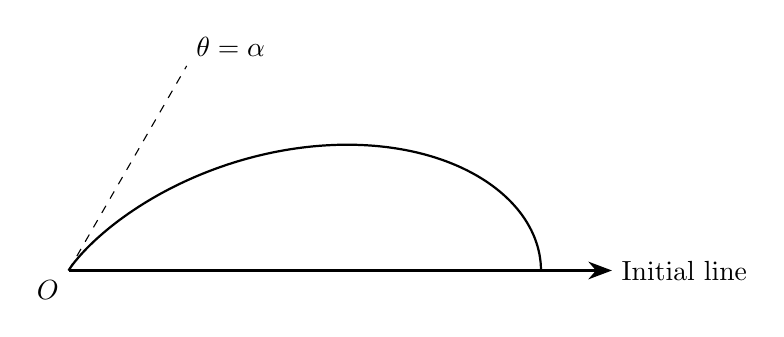
\begin{tikzpicture}[scale=1.5]
\def\radScale{2}
\def\frequency{3}
\pgfmathsetmacro{\alphaDraw}{180/\frequency}
\pgfmathsetmacro{\rayLength}{\radScale}
\pgfmathsetmacro{\axisLength}{2.3*\radScale}
\coordinate (O) at (0,0);
\coordinate (T) at (\alphaDraw:\rayLength);
\coordinate (H) at (\axisLength,0);
\draw[thick, black, domain=0:\alphaDraw, samples=180, variable=\t]
  plot ({\radScale*(1+cos(\frequency*\t))*cos(\t)},{\radScale*(1+cos(\frequency*\t))*sin(\t)});
\draw[thick, black, -{Stealth[length=3mm]}] (O) -- (H);
\draw[dashed, black] (O) -- (T);
\node[below left] at (O) {$O$};
\node[right] at (H) {Initial line};
\node[above right] at (T) {$\theta=\alpha$};
\end{tikzpicture}
\end{figure}


A curve has polar equation
\[
r=2(1+\cos 3\theta),\qquad 0\leq\theta<2\pi
\] \\
with only points for which $r>0$ represented by polar coordinates. The pole $O$ is included as a limiting point of the curve. \\
\begin{enumerate}[label=\textbf{(\roman*)}]
\item The diagram above shows the arc traced from $\theta=0$ until the curve first reaches $O$. The tangent there has equation $\theta=\alpha$, where $0<\alpha<\pi$. Find $\alpha$ in terms of $\pi$. \marks{2} \\
\item
\begin{enumerate}[label=(\alph*)]
\item Let $f(\theta)=2(1+\cos 3\theta)$. Show that, for every integer $k$,
\[
f\left(\frac{2k\pi}{3}-\theta\right)=f(\theta)
\] \\
and also show that
\[
f\left(\theta+\frac{2\pi}{3}\right)=f(\theta)
\] \marks[-30pt]{4}
\item Hence state the equations of all the distinct lines of symmetry of the curve, using angles in $0\leq\theta<\pi$. State also the smallest positive angle through which the curve can be rotated about $O$ and remain unchanged. \marks{3} \\
\end{enumerate}
\item Sketch the complete curve. State its maximum radius and all the corresponding values of $\theta$ in $0\leq\theta<2\pi$. \marks{4} \\
\end{enumerate}

\vspace*{10pt}

\begin{djsSolution}
\begin{enumerate}[label=\textbf{(\roman*)}, start=1]
\item
At the pole, the radius tends to zero. The first positive angle at which this happens satisfies
\begin{align*}
2(1+\cos 3\theta)&=0\\
\cos 3\theta&=-1\\
3\theta&=\pi
\end{align*}

The tangent at the pole is the line through the pole at the angle where \(r=0\), so
\[
\alpha=\dfrac{\pi}{3}
\]

\item
\begin{enumerate}[label=(\alph*), start=1]
\item Using the addition formula for cosine, with \(\cos 2k\pi=1\) and \(\sin 2k\pi=0\) for every integer \(k\):
\begin{align*}
f\left(\dfrac{2k\pi}{3}-\theta\right)
&=2\left[1+\cos\left(2k\pi-3\theta\right)\right]\\
&=2\left[1+\cos 2k\pi\cos 3\theta+\sin 2k\pi\sin 3\theta\right]\\
&=2(1+\cos 3\theta)\\
&=f(\theta)
\end{align*}

Similarly, using the addition formula for cosine:
\begin{align*}
f\left(\theta+\dfrac{2\pi}{3}\right)
&=2\left[1+\cos\left(3\theta+2\pi\right)\right]\\
&=2\left[1+\cos 3\theta\cos 2\pi-\sin 3\theta\sin 2\pi\right]\\
&=2(1+\cos 3\theta)\\
&=f(\theta)
\end{align*}

\item Reflection in a line \(\theta=\beta\) replaces \(\theta\) by \(2\beta-\theta\). The first identity in part (ii)(a) therefore gives symmetry lines \(\beta=\frac{k\pi}{3}\). The distinct lines in the required range are
\[
\theta=0,\qquad \theta=\dfrac{\pi}{3},\qquad \theta=\dfrac{2\pi}{3}
\]

The second identity in part (ii)(a) gives rotational symmetry. Since \(\cos 3\theta\) has smallest positive period \(\frac{2\pi}{3}\), the smallest positive rotation is
\[
\dfrac{2\pi}{3}
\]

\end{enumerate}
\item The sketch should look like:\par\nopagebreak

\begin{tikzpicture}[scale=1.1]
\def\radScale{2}
\def\frequency{3}
\pgfmathsetmacro{\maxRadius}{2*\radScale}
\pgfmathsetmacro{\axisLength}{1.2*\maxRadius}
\coordinate (O) at (0,0);
\coordinate (H) at (\axisLength,0);
\coordinate (P) at (0:\maxRadius);
\coordinate (Q) at (120:\maxRadius);
\coordinate (R) at (240:\maxRadius);
\foreach \centreAngle in {0,120,240} {
  \pgfmathsetmacro{\startAngle}{\centreAngle-180/\frequency}
  \pgfmathsetmacro{\endAngle}{\centreAngle+180/\frequency}
  \draw[thick, black]
    plot[smooth, samples=121, domain=\startAngle:\endAngle, variable=\t]
    ({\radScale*(1+cos(\frequency*\t))*cos(\t)},
     {\radScale*(1+cos(\frequency*\t))*sin(\t)});
}
\draw[thick, black, -{Stealth[length=3mm]}] (O) -- (H)
  node[right] {Initial line};
\foreach \point in {P,Q,R} {
  \fill[black] (\point) circle (1.5pt);
}
\node[above right] at (P) {$\left(4,0\right)$};
\node[above left] at (Q) {$\left(4,\frac{2\pi}{3}\right)$};
\node[below left] at (R) {$\left(4,\frac{4\pi}{3}\right)$};
\node[below left=2pt] at (O) {$O$};
\end{tikzpicture}

The three identical lobes meet at \(O\) and are related by rotations of \(\frac{2\pi}{3}\). The labelled points are given in polar coordinates.

Since \(\cos 3\theta\leq 1\), the radius satisfies
\[
r=2(1+\cos 3\theta)\leq 4
\]

Equality occurs when
\begin{align*}
\cos 3\theta&=1\\
3\theta&=2k\pi\qquad (k\in\mathbb{Z})\\
\theta&=\dfrac{2k\pi}{3}
\end{align*}

Thus the maximum radius and all its corresponding angles in \(0\leq\theta<2\pi\) are
\[
r_{\max}=4,\qquad \theta=0,\ \dfrac{2\pi}{3},\ \dfrac{4\pi}{3}
\]

\end{enumerate}
\end{djsSolution}

\newpage

% ---- Question 9 ----
\questionitem
% [Source: _QBT___Solns__Polar_Coordinates_Basics, Q9]

\begin{enumerate}[label=\textbf{(\alph*)}]
\item The line $L$ has polar equation
\[
r=3\sec\left(\theta-\frac{\pi}{4}\right),\qquad -\frac{\pi}{4}<\theta<\frac{3\pi}{4}
\] \\
Show that its Cartesian equation is $x+y=3\sqrt{2}$. \marks{2} \\
\item The curve $C$ has polar equation
\[
r=5-2\sin 2\theta,\qquad -\pi<\theta\leq\pi
\] \\
Find the exact polar coordinates of all the points of intersection of $L$ and $C$. \\
Fully justify that you have found every point of intersection. \marks{6} \\
\end{enumerate}

\vspace*{10pt}

\begin{djsSolution}
\begin{enumerate}[label=\textbf{(\alph*)}, start=1]
\item Multiplying the polar equation by \(\cos\left(\theta-\frac{\pi}{4}\right)\) and expanding:
\begin{align*}
r\cos\left(\theta-\dfrac{\pi}{4}\right)&=3\\
\dfrac{r\cos\theta+r\sin\theta}{\sqrt{2}}&=3
\end{align*}

Using \(x=r\cos\theta\) and \(y=r\sin\theta\), we obtain
\[
x+y=3\sqrt{2}
\]

\item On \(C\), \(3\leq r\leq7\), so \(r>0\). At an intersection, the equation of \(L\) gives
\[
\cos\left(\theta-\dfrac{\pi}{4}\right)=\dfrac{3}{r}
\]

Using the double angle formula:
\begin{align*}
\sin2\theta
&=\cos\left(2\theta-\dfrac{\pi}{2}\right)\\
&=2\cos^2\left(\theta-\dfrac{\pi}{4}\right)-1\\
&=\dfrac{18}{r^2}-1
\end{align*}

Substituting into the equation of \(C\):
\begin{align*}
r&=5-2\left(\dfrac{18}{r^2}-1\right)\\
r&=7-\dfrac{36}{r^2}\\
r^3-7r^2+36&=0\\
(r-3)(r^2-4r-12)&=0\\
(r-3)(r-6)(r+2)&=0
\end{align*}

Since \(3\leq r\leq7\), the possible radii are \(r=3\) and \(r=6\).
The angular restriction on \(L\) gives
\[
-\dfrac{\pi}{2}<\theta-\dfrac{\pi}{4}<\dfrac{\pi}{2}
\]

For \(r=3\):
\begin{align*}
\cos\left(\theta-\dfrac{\pi}{4}\right)&=1\\
\theta-\dfrac{\pi}{4}&=0\\
\theta&=\dfrac{\pi}{4}
\end{align*}

For \(r=6\):
\begin{align*}
\cos\left(\theta-\dfrac{\pi}{4}\right)&=\dfrac12\\
\theta-\dfrac{\pi}{4}&=\pm\dfrac{\pi}{3}\\
\theta&=-\dfrac{\pi}{12}\quad\text{or}\quad\dfrac{7\pi}{12}
\end{align*}

All transformations above are reversible for \(r>0\), and these are all the solutions of the cosine equations in the allowed interval. All three angles also lie in the domain of \(C\). Hence every intersection has been found, and the exact polar coordinates are
\[
\left(3,\dfrac{\pi}{4}\right),\qquad
\left(6,-\dfrac{\pi}{12}\right),\qquad
\left(6,\dfrac{7\pi}{12}\right)
\]

\end{enumerate}
\end{djsSolution}

\newpage

% ---- Question 10 ----
\questionitem
% [Source: _QBT___Solns__Polar_Coordinates_Basics, Q10]

\begin{enumerate}[label=\textbf{(\alph*)}]
\item The curve $C$ is the right-hand branch of the hyperbola
\[
x^2-y^2=6x,\qquad x\geq6
\] \\
Using $x=r\cos\theta$ and $y=r\sin\theta$, show that its polar equation is
\[
r=6\cos\theta\sec 2\theta,\qquad -\frac{\pi}{4}<\theta<\frac{\pi}{4}
\] \\
where $r>0$. \marks{3} \\

\begin{figure}[H]
    \centering
\begin{tikzpicture}[scale=0.4]
\def\xmax{17}
\def\ymax{12}
\def\ymin{-12}
\def\coef{6}
\pgfmathsetmacro{\halfcoef}{\coef/2}
\coordinate (O) at (0,0);
\coordinate (E) at (\xmax,0);
\begin{scope}
  \clip (0,\ymin) rectangle (\xmax,\ymax);
  \draw[thick, black, samples=200, domain=\ymin:\ymax, variable=\u]
    plot ({\halfcoef+sqrt(\halfcoef*\halfcoef+\u*\u)},{\u});
\end{scope}
\draw[-{Stealth[length=3mm]}, thick, black] (O) -- (E);
\node[below left] at (O) {$O$};
\node[below] at ($(O)!0.75!(E)$) {Initial line};
\end{tikzpicture}
\end{figure}


\item The diagram above shows the curve $C$. \\
\begin{enumerate}[label=(\roman*)]
\item Find the polar coordinates of the point $N$ on $C$ nearest to the pole $O$. Justify that your point gives the minimum value of $r$. \marks{3} \\
\item The circle $r=6\sqrt{3}$ meets $C$ at $P$ and $Q$, where $P$ lies above the initial line and $Q$ lies below it. Find their exact polar coordinates, using angles in the interval $-\frac{\pi}{4}<\theta<\frac{\pi}{4}$. \marks{5} \\
\item Find the exact value, in radians, of the angle $PNQ$. \marks{4} \\
\end{enumerate}
\end{enumerate}

\vspace*{10pt}

\begin{djsSolution}
\begin{enumerate}[label=\textbf{(\alph*)}, start=1]
\item Substituting \(x=r\cos\theta\) and \(y=r\sin\theta\):
\begin{align*}
r^2\cos^2\theta-r^2\sin^2\theta&=6r\cos\theta\\
r^2\cos2\theta&=6r\cos\theta\\
r\cos2\theta&=6\cos\theta
\end{align*}

The last step uses \(r>0\). Since \(x>0\), we may take \(-\frac{\pi}{2}<\theta<\frac{\pi}{2}\), so \(\cos\theta>0\). Thus
\[
\cos2\theta=\dfrac{6\cos\theta}{r}>0
\]

Within this interval, \(\cos2\theta>0\) requires \(-\frac{\pi}{4}<\theta<\frac{\pi}{4}\). Hence the polar equation is
\[
r=6\cos\theta\sec2\theta,\qquad -\dfrac{\pi}{4}<\theta<\dfrac{\pi}{4}
\]

\item
\begin{enumerate}[label=(\roman*), start=1]
\item On the given interval, \(0<\cos\theta\leq1\) and \(\cos2\theta>0\). Therefore
\begin{align*}
\cos2\theta&=\cos^2\theta-\sin^2\theta\leq\cos^2\theta\leq\cos\theta\\
r&=\dfrac{6\cos\theta}{\cos2\theta}\geq6
\end{align*}

Equality occurs only when \(\theta=0\), which gives \(r=6\). Thus \(N\) has polar coordinates
\[
(6,0)
\]

\item At an intersection, \(r=6\sqrt3\). Using the polar equation from part (a):
\begin{align*}
6\sqrt3\cos2\theta&=6\cos\theta\\
\sqrt3(2\cos^2\theta-1)&=\cos\theta\\
2\sqrt3\cos^2\theta-\cos\theta-\sqrt3&=0\\
(2\cos\theta-\sqrt3)(\sqrt3\cos\theta+1)&=0\\
\cos\theta&=\dfrac{\sqrt3}{2}\quad\text{or}\quad-\dfrac{1}{\sqrt3}
\end{align*}

Since \(\cos\theta>0\) on the given interval, the negative value is excluded. Hence \(\theta=\pm\frac{\pi}{6}\). The positive angle gives the point above the initial line, so \(P\) has polar coordinates
\[
\left(6\sqrt3,\dfrac{\pi}{6}\right)
\]

and \(Q\) has polar coordinates
\[
\left(6\sqrt3,-\dfrac{\pi}{6}\right)
\]

\item From the polar coordinates, \(ON=6\), \(OP=6\sqrt3\) and \(\angle NOP=\frac{\pi}{6}\). Applying the cosine rule in triangle \(ONP\):
\begin{align*}
NP^2&=6^2+(6\sqrt3)^2-2(6)(6\sqrt3)\cos\dfrac{\pi}{6}\\
&=36+108-108=36\\
NP&=6
\end{align*}

Since \(ON=NP\), triangle \(ONP\) is isosceles, with \(\angle NPO=\angle NOP=\frac{\pi}{6}\). Therefore
\[
\angle ONP=\pi-\dfrac{\pi}{6}-\dfrac{\pi}{6}=\dfrac{2\pi}{3}
\]

By symmetry about the initial line, \(\angle ONQ=\angle ONP\). Using the angles around \(N\):
\[
\angle PNQ=2\pi-2\left(\dfrac{2\pi}{3}\right)=\dfrac{2\pi}{3}\text{ radians}
\]

\end{enumerate}
\end{enumerate}
\end{djsSolution}

\end{enumerate}
\end{document}
